\documentclass[border=6pt]{standalone}
\usepackage[T1]{fontenc}
\usepackage{libertine}
\usepackage{amsmath}
\usepackage{xcolor}
\usepackage{tikz}
\usetikzlibrary{positioning,fit,backgrounds,arrows.meta,calc}

\definecolor{blueLine}{HTML}{26477E}
\definecolor{blueFill}{HTML}{E8F0FA}
\definecolor{blueBox}{HTML}{F4F8FD}
\definecolor{blueText}{HTML}{1F3F86}
\definecolor{orngLine}{HTML}{CE6A2C}
\definecolor{orngFill}{HTML}{FCF1E9}
\definecolor{orngBox}{HTML}{FEFBF7}
\definecolor{orngText}{HTML}{C0561C}
\definecolor{grnLine}{HTML}{2C6B38}
\definecolor{grnFill}{HTML}{E8F3E8}
\definecolor{grnBox}{HTML}{F5FAF5}
\definecolor{grnText}{HTML}{1D5E2B}
\definecolor{infLine}{HTML}{9A9AA6}
\definecolor{infBox}{HTML}{ECECF2}
\definecolor{infText}{HTML}{33333A}
\definecolor{arrowCol}{HTML}{2A3A55}
\definecolor{topText}{HTML}{202A45}
\definecolor{subText}{HTML}{2D2D2D}

\newcommand{\BX}[3]{{\small\bfseries\color{#1}#2}\\[2.5pt]{\footnotesize\itshape\color{subText}#3}}

\begin{document}
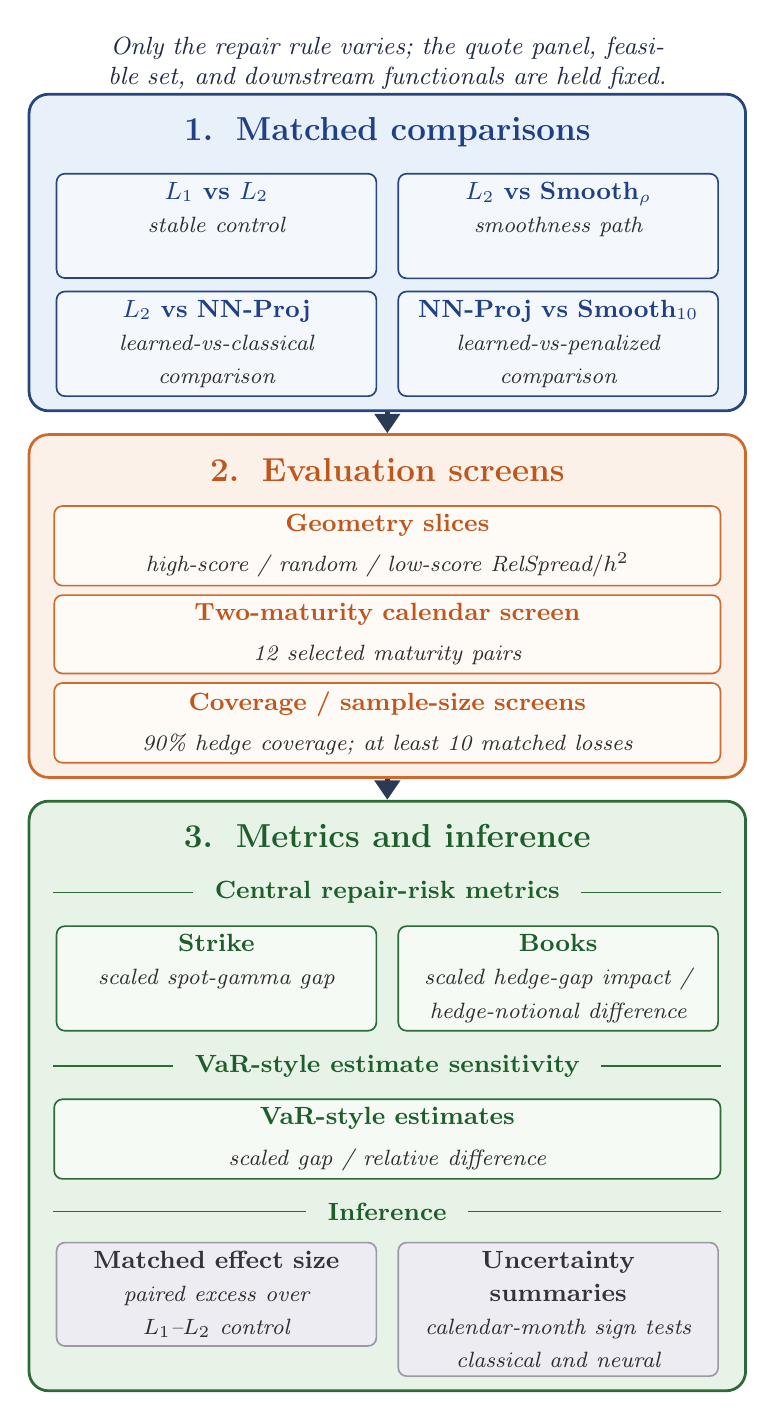
\begin{tikzpicture}[
  ibox/.style={rounded corners=3pt, line width=0.6pt, align=center, inner xsep=4pt, inner ysep=3pt},
  bluebox/.style={ibox, draw=blueLine, fill=blueBox},
  orngbox/.style={ibox, draw=orngLine, fill=orngBox},
  grnbox/.style={ibox, draw=grnLine, fill=grnBox},
  infbox/.style={ibox, draw=infLine, fill=infBox},
  outer/.style={rounded corners=7pt, line width=1pt, inner sep=5pt, minimum width=9.10cm},
  hdr/.style={font=\large\bfseries},
  glabel/.style={font=\small\bfseries, text=grnText},
]

% ===================== top line =====================
\node[font=\small\itshape, text=topText, align=center, text width=8.5cm] (top) at (0,-0.25)
  {Only the repair rule varies; the quote panel, feasible set, and downstream functionals are held fixed.};

% ===================== Section 1 (2x2, legend removed) =====================
\node[hdr, text=blueText, anchor=north] (h1) at (0,-0.82) {1.\, Matched comparisons};

\node[bluebox, text width=3.78cm, minimum height=1.24cm, anchor=north] (s1a) at ($(h1.south)+(-2.17,-0.20)$)
  {\BX{blueText}{$L_1$ vs $L_2$}{stable control\\\vphantom{Mg}}};
\node[bluebox, text width=3.78cm, minimum height=1.24cm, anchor=north] (s1b) at ($(s1a.north)+(4.34,0)$)
  {\BX{blueText}{$L_2$ vs Smooth$_\rho$}{smoothness path\\\vphantom{Mg}}};
\node[bluebox, text width=3.78cm, minimum height=1.24cm, anchor=north] (s1c) at ($(s1a.south)+(0,-0.15)$)
  {\BX{blueText}{$L_2$ vs NN-Proj}{learned-vs-classical\\comparison}};
\node[bluebox, text width=3.78cm, minimum height=1.24cm, anchor=north] (s1d) at ($(s1c.north)+(4.34,0)$)
  {\BX{blueText}{NN-Proj vs Smooth$_{10}$}{learned-vs-penalized\\comparison}};

\begin{scope}[on background layer]
  \node[outer, draw=blueLine, fill=blueFill, fit=(h1)(s1a)(s1b)(s1c)(s1d)] (sec1) {};
\end{scope}

% ===================== Section 2 (stacked, footnote removed) =====================
\node[hdr, text=orngText, anchor=north] (h2) at ($(sec1.south)+(0,-0.46)$) {2.\, Evaluation screens};

\node[orngbox, text width=8.18cm, minimum height=0.82cm, anchor=north] (s2a) at ($(h2.south)+(0,-0.18)$)
  {\BX{orngText}{Geometry slices}{high-score / random / low-score RelSpread$/h^2$}};
\node[orngbox, text width=8.18cm, minimum height=0.82cm, anchor=north] (s2b) at ($(s2a.south)+(0,-0.10)$)
{\BX{orngText}{Two-maturity calendar screen}{12 selected maturity pairs}};
\node[orngbox, text width=8.18cm, minimum height=0.82cm, anchor=north] (s2c) at ($(s2b.south)+(0,-0.10)$)
  {\BX{orngText}{Coverage / sample-size screens}{90\% hedge coverage; at least 10 matched losses}};

\begin{scope}[on background layer]
  \node[outer, draw=orngLine, fill=orngFill, fit=(h2)(s2a)(s2c)] (sec2) {};
\end{scope}

% ===================== Section 3 (footnote removed) =====================
\node[hdr, text=grnText, anchor=north] (h3) at ($(sec2.south)+(0,-0.46)$) {3.\, Metrics and inference};

\node[glabel, anchor=north] (lblA) at ($(h3.south)+(0,-0.18)$) {Central repair-risk metrics};
\node[grnbox, text width=3.78cm, minimum height=1.12cm, anchor=north] (s3strike) at ($(lblA.south)+(-2.17,-0.15)$)
  {\BX{grnText}{Strike}{scaled spot-gamma gap\\\vphantom{Mg}}};
\node[grnbox, text width=3.78cm, minimum height=1.12cm, anchor=north] (s3books) at ($(s3strike.north)+(4.34,0)$)
  {\BX{grnText}{Books}{scaled hedge-gap impact /\\hedge-notional difference}};

\node[glabel, anchor=north] (lblB) at ($(s3strike.south)+(2.17,-0.17)$) {VaR-style estimate sensitivity};
\node[grnbox, text width=8.18cm, minimum height=0.82cm, anchor=north] (s3lim) at ($(lblB.south)+(0,-0.15)$)
  {\BX{grnText}{VaR-style estimates}{scaled gap / relative difference}};

\node[glabel, anchor=north] (lblC) at ($(s3lim.south)+(0,-0.17)$) {Inference};
\node[infbox, text width=3.78cm, minimum height=1.12cm, anchor=north] (s3eff) at ($(lblC.south)+(-2.17,-0.15)$)
  {\BX{infText}{Matched effect size}{paired excess over\\$L_1$--$L_2$ control}};
\node[infbox, text width=3.78cm, minimum height=1.12cm, anchor=north] (s3unc) at ($(s3eff.north)+(4.34,0)$)
  {\BX{infText}{Uncertainty summaries}{calendar-month sign tests\\classical and neural}};

\begin{scope}[on background layer]
  \node[outer, draw=grnLine, fill=grnFill, fit=(h3)(lblA)(s3strike)(s3books)(lblB)(s3lim)(lblC)(s3eff)(s3unc)] (sec3) {};
\end{scope}

% ----- sub-group flanking rules -----
\foreach \lb in {lblA,lblB,lblC}{%
  \draw[grnLine, line width=0.5pt] (s3lim.west |- \lb) -- ($(\lb.west)+(-0.15,0)$);
  \draw[grnLine, line width=0.5pt] ($(\lb.east)+(0.15,0)$) -- (s3lim.east |- \lb);
}

% ----- arrows -----
\draw[arrowCol, line width=1.8pt, -{Triangle[length=7pt,width=9pt]}] (sec1.south) -- (sec2.north);
\draw[arrowCol, line width=1.8pt, -{Triangle[length=7pt,width=9pt]}] (sec2.south) -- (sec3.north);

\end{tikzpicture}
\end{document}
